
\documentclass{article}
\usepackage[utf8]{inputenc}
\usepackage[T1]{fontenc}
\usepackage[frenchb]{babel}
\usepackage[bookmarks=true]{hyperref}
\usepackage{lmodern}
\usepackage{graphicx}
%\usepackage{fullpage}

\author{Gentile Pierre, Didier-Roche François}
\date{\today}
\title{Document de spécification des exigences}

\frenchbsetup{StandardLists=true}
\begin{document}

\maketitle

\newpage
\tableofcontents
\newpage


\section{Introduction}
\subsection{Objet}
Ce document est destiné aux personnes souhaitant connaître toutes les exigences propres au projet. Il détaille en plusieurs parties 
les fonctionnalités de l'application de manière simple et précise. 
\subsection{Portée du projet}
Appointime cherche à faciliter la prise de rendez-vous et l’accès aux disponibilités des artisans/entreprises de services.
Elle permet de mettre en relation des particuliers et des artisans/entreprises de services intuitivement et rapidement.
L’application sera donc divisée en deux: la partie particulier et la partie professionnelle.
\begin{itemize}
\item Le professionnel pourra indiquer son domaine de compétences, les détails de son entreprise, ses disponibilités
ainsi que les prestations qu’il peut effectuer.
\item Tout les utilisateurs pourront faire des recherches selon leurs
  besoins et trouver rapidement et intuitivement des professionnels
  disponibles aux alentours.
\end{itemize}
\subsection{Définitions, acronymes, abréviations}
\begin{itemize}
\item \textbf{Domaines d'activité} : Ici, les domaines d'activité qu'un professionnel pourra spécifier seront prédéfinis par une liste (mécanicien, coiffeur...)

\item \textbf{Prestations} : Ici, ce sont les tâches de base
(qui ont un coût et un temps de travail peu variable) que le professionnel pourra proposer afin de faciliter la réservation.
\item \textbf{Professionnel} : Ce terme décrit toutes les personnes ayant une entreprise proposant des
  prestations sur prise de rendez-vous sur l'application.
\item \textbf{Pariculier} : Ce terme décrit toutes les personnes
  voulant prendre rendez-vous auprès d'un professionnel qui offre un service et des disponibilités correspondant à ses besoins.
\item \textbf{Flashcode} : Un flashcode est un identifiant sous forme
  d'image en 2 dimensions pouvant être lu par l'appareil photo d'un smartphone et
  interprété par un programme.
\item \textbf{Numéro de siret} : Le numéro SIRET (système d'identification du répertoire des établissements) est une série de 14 chiffres.
Cette serie de chiffres identifie l'entreprise ainsi que l'établissement.
\end{itemize}


\subsection{Vue d'ensemble}
Dans ce document, nous décrirons de plus en plus précisément l'application.
Tout d'abord nous nous intéresserons aux principales fonctions de l'application ainsi qu'au profil des utilisateurs.
Ensuite, nous définirons sa structure et son agencement. 
Enfin nous détaillerons les interactions avec l'utilisateur, puis nous préciserons leurs exigences spécifiques.
Pour finir, nous aborderons les exigences de performance puis celles relatives aux bases de données.

\section{Description générale}
\subsection{Environnement}
\begin{itemize}
\item Le système décrit est une application mobile sur IOS et
Android.
\item Le système est adapté pour n'importe quel smartphone ayant IOS (8 ou supérieur) ou Android (6 ou supérieur) comme
système d'exploitation.
\item Les actions de l'utilisateur s'éffectuent via l'écran
  tactile, le capteur d'empreintes digitales ou l'appareil photo du smartphone.
\item L'application communique avec une base de données distante
  via une connexion \og réseau mobile\fg{} ou Wifi.
\subsection{Obtention de l'application}
L'application pourra être obtenue via les marchés d'applications propres aux systèmes d'exploitation cités précédement.
(AppStore et Google Play Store)

%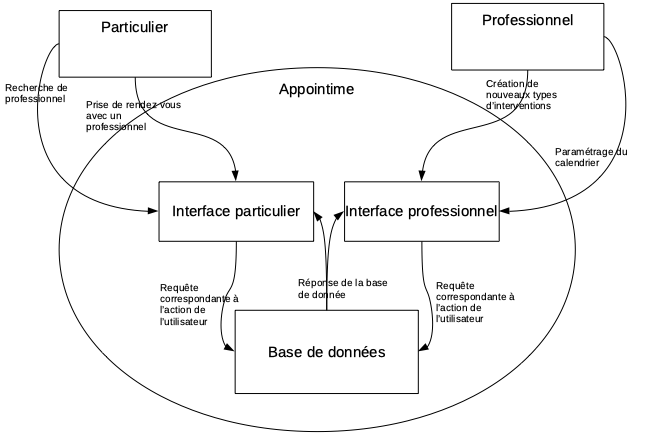
\includegraphics[scale=0.5]{ShematDiagrammes/ShematGeneral.png}
\end{itemize}
\subsection{Fonctions}
\begin{itemize}
\item L'application permet à n'importe quel professionnel de

	\begin{itemize}
	\item renseigner les détails de son entreprise (nom, description du
	domaine d'activité, description générale, numéro de siret),
	\item renseigner sa politique d'annulation par un particulier, de rendez-vous (durée minimale d'annulation nécéssaire pour un remboursement),
	\item renseigner/modifier ses horaires de travail,
	\item créer/modifier/supprimer des prestations qu'il proposera aux particuliers,
	\item inspecter et confirmer/refuser des demandes de rendez-vous formulés par des particuliers.
	\end{itemize}
\item L'application permet à n'importe quel utilisateur de

 	\begin{itemize}
	\item rechercher un professionnel,
	\item prendre un rendez-vous chez un professionnel selon les disponnibilités de
	ce dernier.
	\end{itemize}
\end{itemize}
\subsection{Caractéristiques des utilisateurs}
\begin{itemize}
\item L'utilisateur aura précisé, lors de son inscription, un email, mot
de passe, nom, prénom, numéro de téléphone, adresse.
\item L'utilisateur n'a besoin d'aucune connaissances techniques.
\item L'utilisateur peut être soit un professionnel soit un particulier.
\item Un professionnel devra préciser les détails de son entreprise (nom, description du
	domaine d'activité, description générale, numéro de siret, horaires d'ouverture, prestations, politique d'annulation de rendez-vous).
\end{itemize}
\subsection{Contraintes}
\begin{itemize}
\item La prise et l'annulation de rendez-vous doit se plier à la
  politique de chaque professionnel.
\item Les informations des utilisateurs devront uniquement être
  utilisées dans le cadre de l'application.
\end{itemize}
\subsection{Hypothèses et dépendances}
\subsubsection{Système d'exploitation}
\paragraph{Système d'exploitation Apple}
~~\\Nous supposons que l'application sera utilisée sur une version d'IOS supérieure ou égale à IOS 8.
\paragraph{Système d'exploitation Android}
~~\\ Nous supposons que l'application sera utilisée sur une version d'Android supérieure ou égale à Android 6.0.
\subsubsection{Accès au réseau}
Nous supposons que les appareils utilisant l'application seront reliés à internet.

\section{Exigences spécifiques}
\subsection{Exigences des interfaces externes}
\subsubsection{Interfaces avec les utilisateurs}
\paragraph{Le menu déroulant:}
Un menu déroulant sera présent en haut à droite de l'interface afin de faciliter la navigation.
\begin{center}
  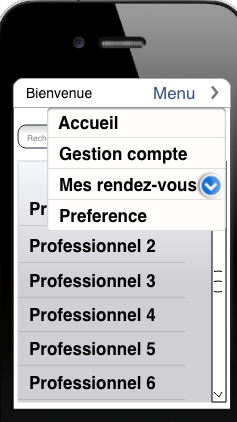
\includegraphics[width=100pt]{user}
  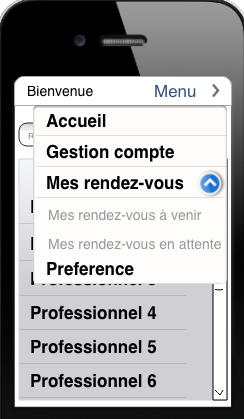
\includegraphics[width=100pt]{deplie}
  \\Les images ci-dessus sont des croquis et non les interfaces finales.
\end{center}
Ainsi un utilisateur pourra accéder


\begin{itemize}
\item à l'accueil via un bouton \og Accueil \fg{},
\item à ses préférences via le bouton \og Préférences \fg{},
\item à ses informations personnelles via un bouton\og Gérer mon compte \fg{},
\item à des nouveaux boutons en appuyant sur \og Mes rendez-vous \fg{}, permettant d'accéder à :
	\begin{itemize}
	\item La liste de ses rendez-vous à venir via un bouton \og Mes rendez-vous à venir \fg{},
	\item La liste de ses rendez-vous en attente de confirmation via un bouton \og En attente de confirmation \fg{}.
	\end{itemize}
	
	




\end{itemize}
Un professionnel pourra accéder aux fonctionnalités citées ci-dessus ainsi que :
\begin{itemize}
\item à des nouveaux boutons en appuyant sur \og Mon entreprise \fg{}, permettant d'accéder à :
\begin{itemize}
\item La page visible par les particuliers via un bouton \og Ma fiche de professionnel \fg{},
\item La page de gestion des horaires via le bouton \og Gérer les horaires d'ouverture \fg{},
\item La page de gestion des prestations via le bouton \og Mes prestations \fg{},
\end{itemize}
\item à des nouveaux boutons en appuyant sur  \og Rendez-vous reçus \fg{}, permetant d'accéder à :
\begin{itemize}
\item La page de gestion des rendez-vous reçus non traités via un bouton \og Gestion des nouvelles demandes \fg{},
\item La page d'affichage du calendrier de rendez-vous via un bouton \og Mon calendrier de rendez-vous \fg{}.
\end{itemize}
\end{itemize}
\begin{center}
  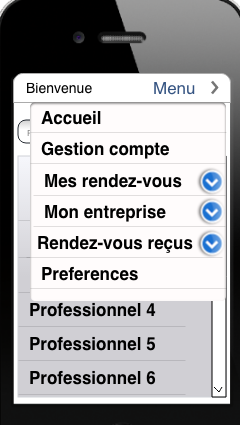
\includegraphics[width=100pt]{pro}
  \\L'image ci-dessus est un croquis et non l'interface finale.
\end{center}
\paragraph{Les informations des utilisateurs :}
\begin{itemize}
 \item Un formulaire d'inscription doit permettre à l'utilisateur de
   s'inscrire en entrant différents champs textuels (email,
   confirmation de l'email, mot de
   passe, confirmation du mot de passe, nom, prénom, numéro de téléphone, adresse) nécéssaires au
   système , et en appuyant sur
   un bouton \og S'inscrire en tant que professionnel\fg{} ou \og S'inscrire en tant que particulier\fg{} selon le besoin de l'utilisateur.

%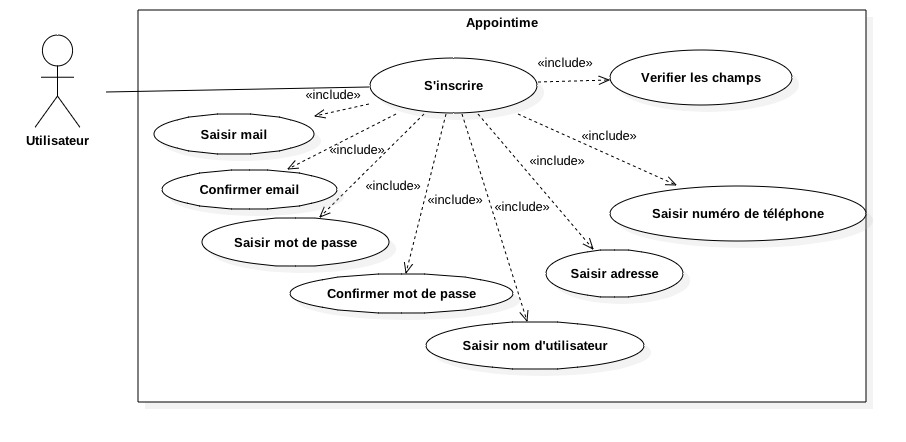
\includegraphics[scale=0.5]{ShematDiagrammes/useCaseInscription.jpg}
\item Si l'utilisateur a choisi l'inscription en tant que professionnel, un formulaire (disponible par redirection
directement après l'inscription et/ou via le menu de navigation) doit lui permettre de renseigner les informations relatives
à son entreprise (nom, description du domaine d'activité, description générale, numéro de siret, politique d'annulation).

\item Si l'utilisateur est un professionnel : un formulaire, accessible via le menu de navigation, doit lui permettre de renseigner les informations relatives aux
horaires d'ouverture de son entreprise (heure d'ouverture et fermeture pour chaque demi-journée (matin/après midi) de la semaine).

\item Un formulaire, accessible via le menu de navigation, doit permettre à un utilisateur de modifier les
  informations mentionnées durant son inscription.
\item Un formulaire de connexion doit permettre à un utilisateur de
  s'identifier pour avoir accès aux services du système en entrant
  différents champs textuels (email, mot de passe) et en appuyant sur
  un bouton \og Se connecter \fg{}.

\item Une reconnaissance par empreinte digitale doit permette à un
  utilisateur de pouvoir s'identifier rapidement dans le cas où cette
  fonctionnalité est diponible sur le téléphone.
\item Une reconnaissance faciale doit permette à un
  utilisateur de pouvoir s'identifier rapidement dans le cas où cette
  fonctionnalité est diponible sur le téléphone.
\end{itemize}

\paragraph{Préférences des utilisateurs :}
\begin{itemize}
\item L'utilisateur doit pouvoir accéder à la page \og Paramètres \fg{} de l'application via le menu
 puis en sélectionnant \og Préférences \fg{}
  dans ce dernier.
\item L'utilisateur doit pouvoir activer ou désactiver les notifications
  de l'application dans le menu paramètres.
\item L'utilisateur doit pouvoir modifier le son des notifications
  (volume et tonalité) dans la page paramètres.
\item L'utilisateur doit pouvoir activer le thème nuit, qui modifie les
  couleurs de l'application, dans la page paramètres.
\item L'utilisateur, s'il est professionnel, doit pouvoir activer la notification par sms.
\end{itemize}
\paragraph{Recherche d'un professionnel :}
\begin{itemize}
\item Un champs textuel doit permettre à l'utilisateur d'effectuer une
  recherche par mot clef (nom d'entreprise, secteur d'activité, domaine d'activité, numéro de siret) ou via un flashcode fourni par le professionnel. Dans
  le premier cas, l'utilisateur doit pouvoir sélectionner
  un périmètre maximal de recherche s'il le souhaite.
\item Après avoir fait une recherche, le client doit pouvoir sélectionner un
  professionnel dans la liste affichée.
\item Le particulier doit pouvoir ajouter un professionnel en favoris grâce
  à un bouton présent sur la page dédiée à un professionnel et sur la
  liste déroulante de recherche.

%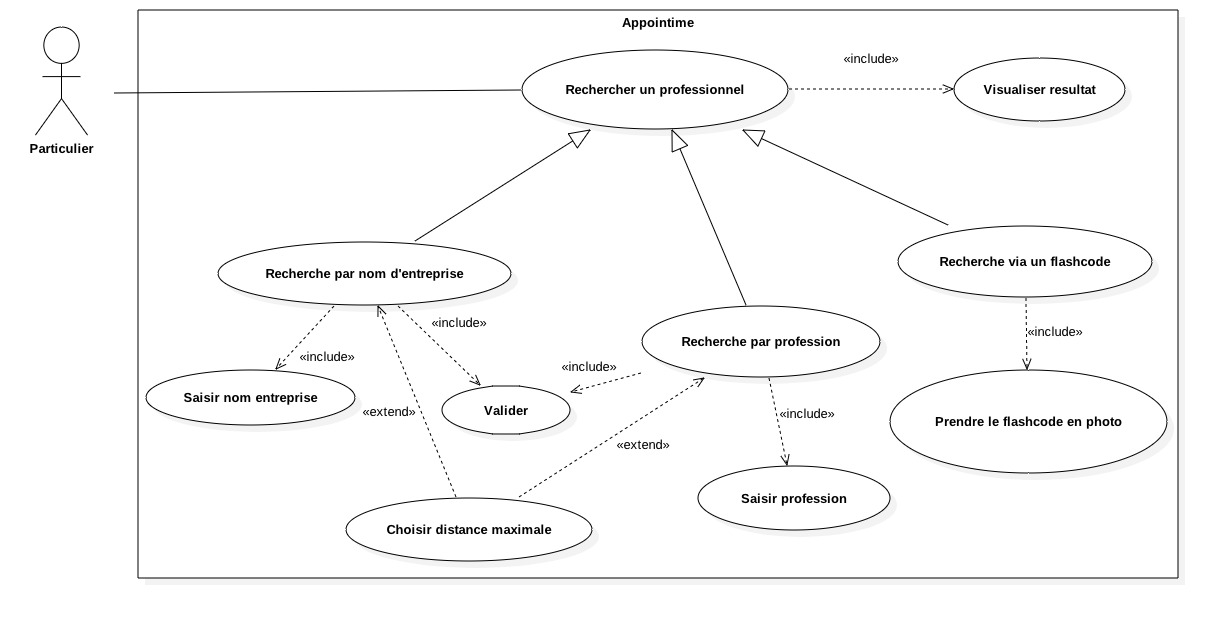
\includegraphics[scale=0.3]{ShematDiagrammes/useCaseRecherchePro.jpg}

\end{itemize}

\paragraph{Prise de rendez-vous chez un professionnel :}
\begin{itemize}

\item La séléction d'un
  professionnel de la liste affichée après une recherche doit permettre d'afficher la
  page dédiée au professionnel en question.
\item Le client doit pouvoir sélectionner une prestation parmi une liste
  proposée par le professionnel.
\item Après avoir selectionné une prestation, le système affiche le
  calendrier du professionnel avec les créneaux diponibles que le
  client peut selectionner.
\item Une fois le créneau sélectionné, le client est redirigé vers
    une page récapitulative de sa prise de rendez-vous (date, heure, details du service, lieu), avec un bouton
    confirmer ou annuler.
\item Si le particulier confirme son choix, les détails de ce rendez-vous s'ajouteront à la liste des rendez-vous 
en attente de confirmation dans la page "en attente de confirmation"
(si la tâche n'est pas en confirmation automatique, sinon, ils seront directement placés dans la section "rendez-vous à venir").
\item Les rendez-vous confirmés par les deux parties (particulier et professionnel) seront listés dans la section "rendez vous à venir"
\item Lors de sa réservation, le client doit pouvoir procéder au
  paiement directement sur l'application si le rendez-vous est confirmé et si le professionnel accepte ce genre de paiement.
\item Le client doit pouvoir ajouter des
  rappels de rendez-vous. Pour ajouter un rappel de rendez-vous, le
  client appuie sur \og Ajouter un rappel \fg{} puis choisit quand le
  rappel va être fait (en nombre d'heures ou de jours avant le
  rendez-vous). Cette fonctionnalité est accessible via un bouton
  prévu à cet effet sur chaque rendez-vous à venir dans la section "Rendez-vous à venir".

%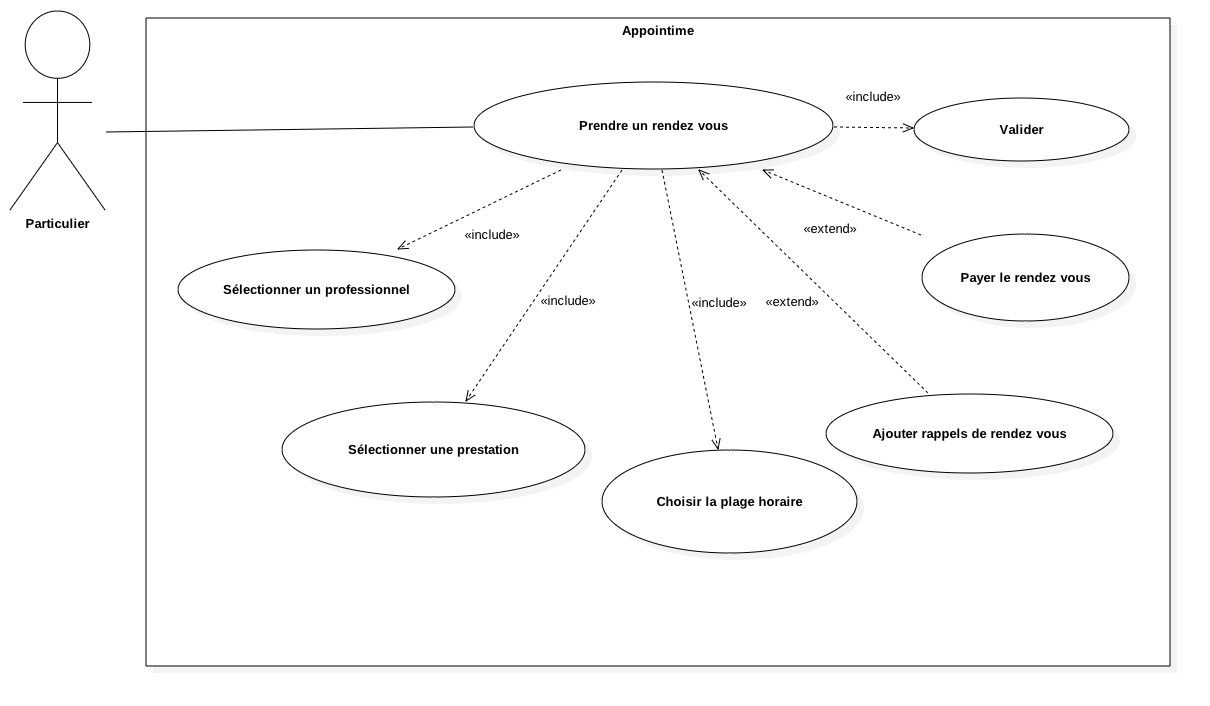
\includegraphics[scale=0.3]{ShematDiagrammes/useCasePriseRdv.jpg}


\end{itemize}

\paragraph{Les informations liées aux rendez-vous :}
~~\\Tous les utilisateurs:
\begin{itemize}
\item L'utilisateur aura accès à la liste de ses rendez-vous à venir via le menu en selectionnant \og Rendez-vous à venir \fg{}.
Il pourra y voir les rendez-vous confirmés par le professionnel qui ne sont pas encore passés.

\item L'utilisateur aura accès à la liste de ses rendez-vous en attente de confirmation via le menu en selectionnant \og En attente de confirmation \fg{}.
Il pourra y voir les rendez-vous en attente de confirmation par le professionnel.


\end{itemize}
Uniquement les professionnels:
\begin{itemize}
\item L'utilisateur aura accès à la liste de ses rendez-vous à confirmer via le menu en selectionnant \og Rendez vous à confirmer \fg{}.
Il pourra y voir les rendez-vous demandés par les particuliers qui ne sont pas encore confirmés.

\end{itemize}

\paragraph{Paramétrage des prestations côté professionnel :}
~~\\Pour l'accès à cette section, voir les details du menu plus haut.
\begin{itemize}
\item Une liste déroulante doit permettre à l'utilisateur d'afficher
  les prestations déjà existantes. Chaque elément de la liste est
  accompagné des boutons \og Sélectionner \fg{}, \og Modifier \fg{} et
  \og Supprimer \fg{}.

\item Un bouton doit permettre au professionnel de créer une nouvelle
  prestation en appuyant sur un bouton \og Ajouter une prestation
  \fg{}.

\item Un formulaire doit permettre de créer une prestation. Ce
  formulaire doit contenir les champs textuels suivant \og Nom \fg{}, \og Description
 \fg{},  \og Durée \fg{}, \og Prix \fg{} et \og Validation automatique \fg{}.

%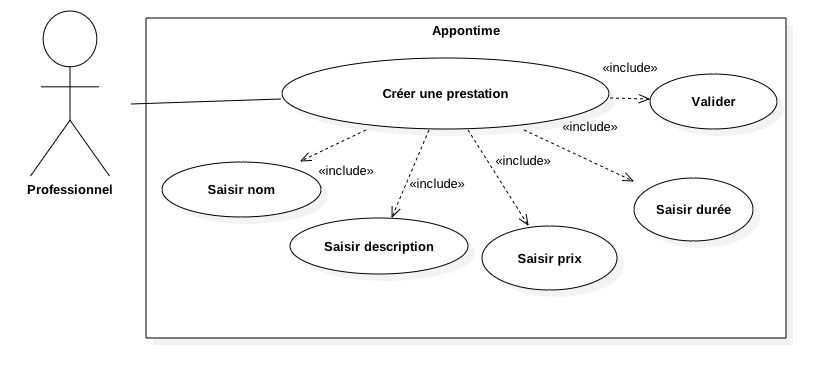
\includegraphics[scale=0.5]{ShematDiagrammes/useCaseCreerPrestation.jpg}

\item Un formulaire doit permettre d'éffectuer des modifications sur
  une prestation. Ce formulaire doit contenir un champ nom, un champ description, un champ
  durée, un champ prix et un champ validation automatique.
\item L'utilisateur doit pouvoir choisir s'il souhaite une validation automatique ou manuelle des rendez-vous.
\end{itemize}
\paragraph{Gestion du calendrier de disponibilités}
\begin{itemize}
\item Un calendrier modifiable doit permettre à l'utilisateur de
  modifier ses diponibilités en modifiant les jours et les horaires
  auxquels il peut effectuer ses prestations.
\item Le calendrier modifiable doit pemettre à l'utilisateur de
  visualiser et de gérer les rendez-vous déjà pris. Sur un créneau
  réservé il doit afficher les informations de l'utilisateur qui a pris
  le rendez-vous ainsi que la prestation qu'il demande. Il doit aussi permettre au professionnel de valider
  ou non les rendez-vous.
\end{itemize}
\paragraph{Acceptation de prise de rendez-vous}
~~\\

Lorsqu'un rendez-vous est pris par un particulier, le
  professionnel reçoit une notification. Lorsque le professionnel
  appuie sur cette dernière, l'application s'ouvre sur une page où sont
  indiqués les informations de l'utilisateur et de la tâche à effectuer.
  Le professionnel pourra accéder à cette demande via le menu (voir le paragraphe dédié au menu plus haut).
\begin{itemize}
\item  Si la prestation est en validation manuelle : un bouton \og
  Accepter le rendez-vous \fg{} et un bouton \og
  Refuser le rendez-vous \fg{} seront présents dans la page décrite précédemment.
\end{itemize}
\paragraph{Signalement des particuliers}
\begin{itemize}
\item Si un rendez-vous a été pris par un particulier mais que ce dernier
  ne s'y est pas rendu, le professionnel doit pouvoir
  signaler le particulier via un bouton \og Signaler \fg{} situé
  sur la page des détails de la réservation. 
  Cette action retire un \og point de crédibilité \fg{} à l'utilisateur qui possède
  3 \og points de crédibilité \fg{}. Si l'utilisateur arrive à 0 point de crédibilité son compte est
  bloqué définitivement. L'utilisateur peut récupérer un point de crédibilité  en étant
  allé à 10 rendez-vous d'affilé.
\end{itemize}

\subsubsection{Interfaces avec les logiciels}
\paragraph{Gestion des notifications :}
L'application doit communiquer avec le système d'exploitation du
smarphone afin d'afficher, lorsque ceci est nécessaire, des
notifications dans la barre de notifications du smartphone.

\subsubsection{Interface avec le materiel}
\paragraph{Identification par empreinte :}
~~\\
L'application doit communiquer avec le materiel si celui-ci dispose
d'un capteur d'empreinte digitale afin de pouvoir se connecter rapidement à
l'application grâce à ce mode d'identification.
\paragraph{Identification par reconnaissance faciale :}
~~\\
L'application devrait communiquer avec le materiel, si celui-ci dispose
d'une technologie de reconnaissance faciale, afin de pouvoir se
connecter rapidement à l'application grâce à ce mode
d'identification.
\paragraph{Recherche par flashcode :}
\begin{itemize}
\item Pour pouvoir être recherché rapidement, chaque professionnel
  doit posséder un flashcode unique.
\item Le particulier doit pouvoir rechercher un professionnel par le
  biais de son appareil photo via un flashcode fourni par le
  professionnel.
\end{itemize}

\subsubsection{Interface de comunication :}
L'application doit communiquer avec un serveur distant via internet
(Wifi ou réseau mobile) contenant la base de données de l'application et
les photos de profil des utilisateurs.


\subsection{Exigences fonctionnelles}
\paragraph{Pour la connexion : }

\begin{itemize}
\item Si l'email existe dans la base de données :
	le système doit vérifier si le mot de passe saisi
	correspond à l'email saisi.
		\begin{itemize}
		\item S'il correspond, le système doit autoriser la connexion et
			rediriger l'utilisateur à l'accueil. Ce dernier aura accès à son
			profil ainsi qu'aux pages de réservation si c'est un particulier et de gestion d'entreprise
			si c'est un professionnel.
		\item S'il ne correspond pas, le système doit afficher une erreur
			et renvoyer sur la page de connexion.
		\end{itemize}
\item S'il n'existe pas le système doit renvoyer une erreur
	et renvoyer sur la page de connexion.
\end{itemize}

%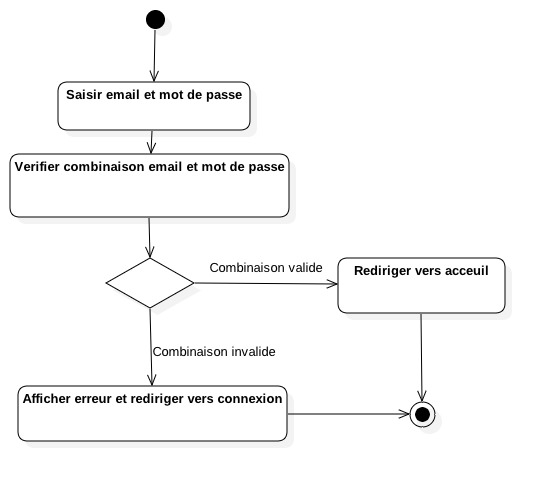
\includegraphics[scale=0.6]{ShematDiagrammes/activiteConnexion.jpg}

\paragraph{Pour l'inscription d'un utilisateur : }
\begin{itemize}
\item Le système doit verifier si les données saisies sont valides
	\begin{itemize}
	\item Si les données sont valides, le système doit vérifier si le mail
		est deja existant.
		\begin{itemize}
		\item Si l'email n'existe pas encore dans la base de données, le système
			doit les enregister, indiquer le bon déroulement de l'opération via un message temporaire et rediriger
			 vers la page de connexion.
		\item Si l'email existe déjà, le système doit rediriger vers
			la page d'inscription et indiquer que le mail est déja utilisé
			via un message.
		\end{itemize}
	\end{itemize}
\item Si les données ne sont pas valides le système doit l'indiquer
	via un message détaillant les erreurs.
\end{itemize}

%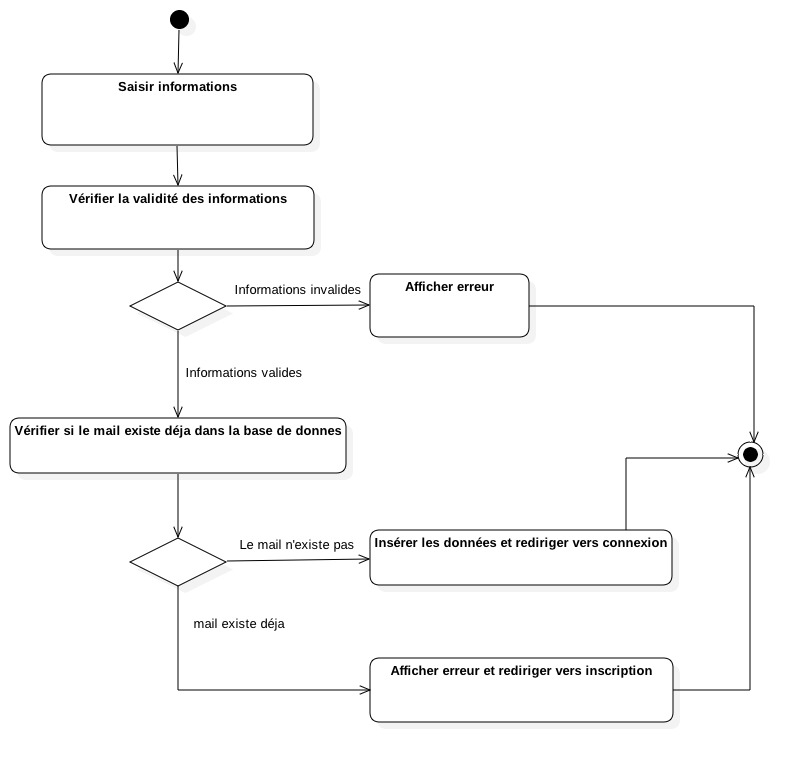
\includegraphics[scale=0.5]{ShematDiagrammes/activiteInscription.jpg}
\paragraph{Pour l'inscription d'une entreprise : }
\begin{itemize}
\item Le système doit vérifier si les données saisies sont valides :

		\begin{itemize}
		\item Si le numéro de siret n'est pas encore utilisé, le système
			doit enregistrer les données, indiquer le bon déroulement de l'opération via un message temporaire et rediriger vers la page de gestion d'horaires d'ouverture.
		\item Si le numéro de siret existe déjà, le système doit rediriger vers
			la page d'inscription d'entreprise et indiquer que le numéro de siret est déja utilisé
			via un message.
		\end{itemize}

\item Si les données ne sont pas valides le système doit l'indiquer
	via un message détaillant les erreurs.
\end{itemize}

\paragraph{Pour la gestion d'horaires d'ouverture d'une entreprise : }
\begin{itemize}
\item Le système doit vérifier si les données saisies sont valides :

		\begin{itemize}
    	\item Si les données sont valides le système
			doit enregistrer les données, indiquer le bon déroulement de l'opération via un message temporaire et rediriger vers la page de gestion d'horaires d'ouverture.
		\item Si les données ne sont pas valides (heure d'ouverture supérieure à l'heure de fermeture, l'heure ne correspond pas à la demi-journée (matin/après midi)) le système doit rediriger vers
			la page de gestion d'horaires d'ouverture et indiquer les erreurs
			via un message.
		\end{itemize}

\item Si les données ne sont pas valides le système doit l'indiquer
	via un message détaillant les erreurs.
\end{itemize}


\paragraph{Pour la gestion de compte : }
\begin{itemize}
\item Le système doit verifier si les données saisies sont valides
	\begin{itemize}
	\item Si les données sont valides :
		\begin{itemize}
		\item Le système remplace les données obsolètes par
                  les nouvelles données.
                \item Le système renvoie l'utilisateur vers la page d'accueil
                 après avoir indiqué via un message temporaire le bon déroulement de l'opération.
		\end{itemize}
		\item Si les données ne sont pas valides :
		\begin{itemize}
		\item Le système renvoie un message d'erreur décrivant
                  les erreurs.
                \item Le système renvoie l'utilisateur sur la page de
                  gestion de compte.
		\end{itemize}
	\end{itemize}
\end{itemize}

\paragraph{Format / validité des données saisies :}
\begin{itemize}
\item L'email et la confirmation d'email sont valides s'ils sont jugés comme des emails.

\item Le mot de passe et la confirmation de mot de passe sont valides s'ils contiennent entre 8 et 25
  caractères et s'ils contiennent au moins une majuscule et une minuscule.

\item Le nom d'utilisateur est valide s'il contient entre 3 et 10
  caractères.

\item Le numéro de téléphone est valide s'il est composé d'exactement
  10 chiffres.

\item L'adresse est valide si elle est composée uniquement de lettres,
  de chiffres et de ponctuation.
\end{itemize}


\paragraph{Pour l'ajout de prestation :}
\begin{itemize}
\item Le système doit verifier si les données saisies sont valides
	\begin{itemize}
	\item Si les données sont valides :
		\begin{itemize}
		\item Le système doit insérer les nouvelles données en base
                  de données,
                 \item le système doit rediriger l'utilisateur vers
                    la page de gestion des prestations.
		\end{itemize}
		\item Si les données ne sont pas valides :
		\begin{itemize}
		\item Le système renvoie un message d'erreur décrivant
                  les erreurs.
                \item Le système doit renvoyer l'utilisateur vers le
                  formulaire d'ajout de prestation.
		\end{itemize}
	\end{itemize}
\end{itemize}


\paragraph{Pour la réservation (coté particulier) :}
Avant la confirmation :
	\begin{itemize}
	\item Si le particulier confirme sa réservation, le système doit :
	\begin{itemize}
	\item Si la tâche n'est pas en confirmation automatique :
		\begin{itemize}
		\item Passer la plage horaire en "en attente de confirmation"
			(la plage horaire ne doit plus être réservable jusqu'à nouvel ordre).
		\item Ajouter la réservation (date, heure, lieu, type de réservation, durée, prix estimé) dans la section "en attente de confirmation"
		\end{itemize}
		\end{itemize}
	\end{itemize}
Apres la confirmation le système doit :
		\begin{itemize}
		\item enregistrer les éventuels changements faits par le professionnel.
		\item déplacer la réservation de "en attente de confirmation" vers "rendez-vous à venir"
		\end{itemize}


\paragraph{Pour la réservation (coté professionnel) :}
\begin{itemize}
\item Avant la confirmation le système doit :
	\begin{itemize}
	\item Ajouter la réservation dans la section "réservations à confirmer" du  professionnel.
    \item Notifier le professionnel d'une demande de réservation via mail, notification sur l'application et éventuellement sms (si le proféssionnel a confirmé l'option prévue à cet effet).
		La notification doit comprendre les informations sur cette reservation (date, heure, lieu, type de réservation, durée, prix estimé)
		ainsi que des informations sur le particulier (profil, points de crédibilité, numéro de téléphone)
	\end{itemize}
\item Pour la confirmation (si elle n'est pas automatique) :
	\begin{itemize}
	\item Le système doit placer la réservation dans la section "rendez vous à venir" et la supprimer de "réservations à confirmer"
	\end{itemize}
\end{itemize}

%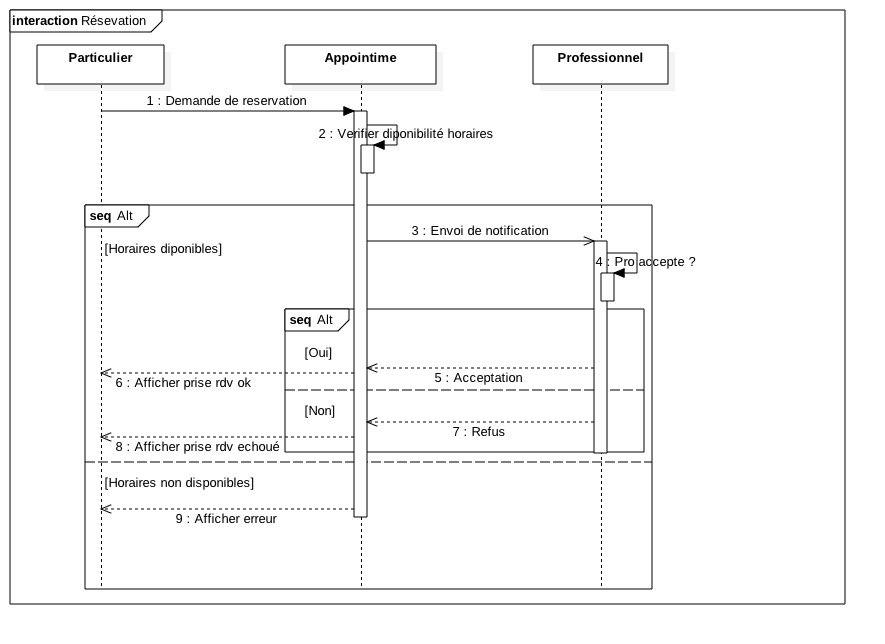
\includegraphics[scale=0.5]{ShematDiagrammes/sequenceReservation.jpg}





\paragraph{Pour la gestion du calendrier du professionnel :}
\begin{itemize}
\item Le système doit verifier la validité des horaires rentrés par l'utilisateur.
\item Le système doit enregistrer les horaires du professionnel dans
  la base de données .
\item Le système doit enregistrer dans la base de données les prestations que le professionnel souhaite ajouter.
\end{itemize}

\paragraph{Rappel de rendez-vous :}
\begin{itemize}
\item Le système doit enregistrer dans une base de données locale les
  rappels de rendez-vous définis par les utilisateurs.
\item Le système doit afficher une notification et émettre un son
  et/ou une vibration lorsque le l'heure du rappel de rendez-vous est
  égale à l'heure du terminal.
\item Le système doit ajouter une notification spéciale définie
  comme suit :
  \begin{itemize}
    \item Le système calcule le temps de voyage approximatif en minute
      noté X que le
      client mettra pour se rendre à son rendez-vous en voiture.
     \item Le système envoie alors une notification X+10 minutes avant
       le rendez-vous.
     \item Cette notification contient le nom du rendez-vous ainsi
       qu'une proposition d'itineraire GPS.
  \end{itemize}

\end{itemize}

\subsection{Exigences de performance :}
\subsubsection{Exigences statiques :}
\paragraph{Taille de l'application :}
L'application ne doit pas excéder 100Mo.
\paragraph{Nombre d'utilisateurs simultanés :}
L'application doit pouvoir supporter 50 utilisateurs/terminaux
simultanément.
\paragraph{Volume de données :}
Le système doit pouvoir dédier 20Mo par utilisateurs soit un total de
1000Mo pour au moins 50 utilisateurs.
\paragraph{Type des données :}
Le système doit pouvoir stocker des données de type entier, chaine de
caractères, booléen et une image 100x100 pixel par utilisateur
(photo de profil).


\subsubsection{Exigences dymamiques :}
\paragraph{Acces au serveur :}
Le système doit permettre un minimum de 50 requêtes/réponses au serveur
par secondes.
\paragraph{Temps de latence :}
\begin{itemize}
\item En condition favorable (50 requêtes/réponses par seconde) le
  système doit avoir un temps de latence maximal de 2 secondes dans
  90\% des cas.
\item En condition de surcharge du serveur (150 requêtes/réponses par
  seconde) le système doit avoir un temps de latence maximal de 4
  secondes dans 75\% des cas.
\end{itemize}

\paragraph{Temps d'execution des tâches hors ligne :}
Le temps de calcul d'une tâche simple sans accès au serveur (exemple : passage d'une vue à
une autre) doit être de 500 milisecondes maximum sur 65\% des
smartphones.

\paragraph{Temps pour une prise de rendez-vous :}
Étant donné un utilisateur ayant utilisé l'application pendant 1
semaine, le temps moyen pour une prise de rendez-vous doit être dans
60\% des cas inférieur à 5 minutes.

\subsection{Exigences logiques relatives aux bases de données}
\subsubsection{Types d'informations utilisées}
\paragraph{Utilisateurs}
~~\\
Pour les utilisateurs, nous devrons stocker :
\begin{itemize}
\item Un identifiant (entier)
\item L'email (chaîne de caractères (entre 5 à 30 caractères))
\item Le nom de l'utilisateur (chaîne de caractères (entre 3 et 20 caractères))
\item le prénom de l'utilisateur (chaîne de caractères (entre 3 et 20 caracteres))
\item Le mot de passe (chaîne de caractères (entre 8 et 25 caractères))
\item Le numéro de téléphone (chaîne de caractères (exactement 10 caractères)
\item L'adresse (chaîne de caractères (maximum 100 caractères))
\item Le fait que l'utilisateur soit professionnel ou non (booléen)
\item Ses points de crédibilité (entier, 3 maximum)
\end{itemize}

\paragraph{Entreprise}
~~\\
Pour les entreprises, nous devrons stocker:
\begin{itemize}
\item Un identifiant (entier)
\item Une référence vers un utilisateur professionnel (id du professionnel(entier))
\item Une description du domaine d'activité (chaîne de caractères (maximum 100 caractères))
\item Une adresse (chaîne de caractères (maximum 100 caractères))
\item Une description générale (chaîne de caractères (maximum 100 caractères))
\item Une description de la politique d'annulation de rendez-vous (chaîne de caractères (maximum 100 caractères))
\item Un numero de siret (chaîne de caractères (14 caractères))
\end{itemize}


\paragraph{Favoris}
~~\\
Pour les favoris, nous devrons stocker:
\begin{itemize}
\item Une référence vers un utilisateur (id de l'utilisateur(entier))
\item Une référence vers une entreprise (id de l'entreprise (entier))
\end{itemize}

\paragraph{Prestations}
~~\\
Pour les prestations, nous devrons stocker
\begin{itemize}
\item Un identifiant (entier)
\item Une référence vers une entreprise (id de l'entreprise (entier))
\item Un titre (chaîne de caractères (maximum 20 caractères))
\item Une description générale (chaîne de caractères (maximum 100 caractères))
\item Une durée d'exécution (entier, en nombre de minutes)
\item Un prix (entier)
\item Une confirmation automatique (booléen)
\end{itemize}

\paragraph{Calendrier}
~~\\
Pour les calendriers, nous devrons stocker
\begin{itemize}
\item Un identifiant (entier)
\item Une référence vers une entreprise (id de l'entreprise (entier))
\item Un numéro de demi-journée de la semaine (entier)
\item Une heure de début de service (date)
\item Une heure de fin de service (date)
\item Un indicateur d'ouverture (booléen)
\end{itemize}

\paragraph{Rendez-vous}
~~\\
Pour les rendez-vous, nous devrons stocker
\begin{itemize}
\item Un identifiant (entier)
\item Une référence vers un utilisateur particulier (id du particulier (entier))
\item Une référence vers une entreprise (id de l'entreprise (entier))
\item Une référence vers une prestation (id de la prestation (entier))
\item L'heure de début (date)
\item L'heure de fin (date)
\end{itemize}


\end{document}
